\documentclass[titlepage]{article}
\usepackage{graphicx}
\usepackage{fancyhdr}
\title{projeye kargah}
\author{Ali jabbari pour}
\date{Due: 6 bahman}
\pagestyle{fancy}
\begin{document}
\maketitle
\tableofcontents
\newpage
\section{sections:}
\begin{enumerate}
    \item Git and GitHub
    \item Exploration Tasks
    \item Git and FOSS
\end{enumerate}
\fancyhead[L]{\thepage}
\newpage
\section{Git and GitHub}
\subsection{Repository Initialization and Commits}
\paragraph{\fontfamily{PM}\selectfont first i made a new repository in my git hub then i made my own new file in my
 desktop and i opened cmd and went to that file using cd then i clone that new repository to this file with git clone}
 \subsection{GitHub Actions for LaTeX Compilation }
 \paragraph{\fontfamily{PM}\selectfont tozihato////benevis}
 \section{Exploration Tasks}
 \subsection{Vim Advanced Features}
 \paragraph{\fontfamily{PM}\selectfont 1-command-driven system 2-plugin support 3-cross-platform compatibility}
 \subsection {Memory profiling}
 \subsubsection{Memory Leak}
 \paragraph{Memory leaks occur when a program allocates memory dynamically but fails to release it after its no longer needed.}
 \subsubsection{Memory profilers }
 \paragraph{valgrind is a powerful tool used to detect memory errors,memory usage mistakes,and performance issues in c and c++programs.
 by running the program in a simulated environment ,valgrind helps programs identify memory leaks and access errors.}
 \subsection{GNU/Linux Bash Scripting}
 \subsubsection{fzf}
 \paragraph{fuzzy searching is a technique used in information retrieval to find results that are
  approximately relevant to a given search query ,even if the query contains errors,misspellings or variations.}
  \paragraph{ls command shows the list of directories and files and fzf
   command let us to search in the list which we achieved with ls command}
\subsubsection{Using fzf to find your favorite PDF}
\paragraph{1-fd -e PDF 2-fd -e pdf | fzf}
\subsubsection{Opening the file using Zathura}
\paragraph{Zathura"\$(fd -e pdf | fzf)"}
\section{Git and FOSS}
\subsubsection{README.md}
\paragraph{done!}
\subsection{Issues}
\begin {figure}[ht]
\centering
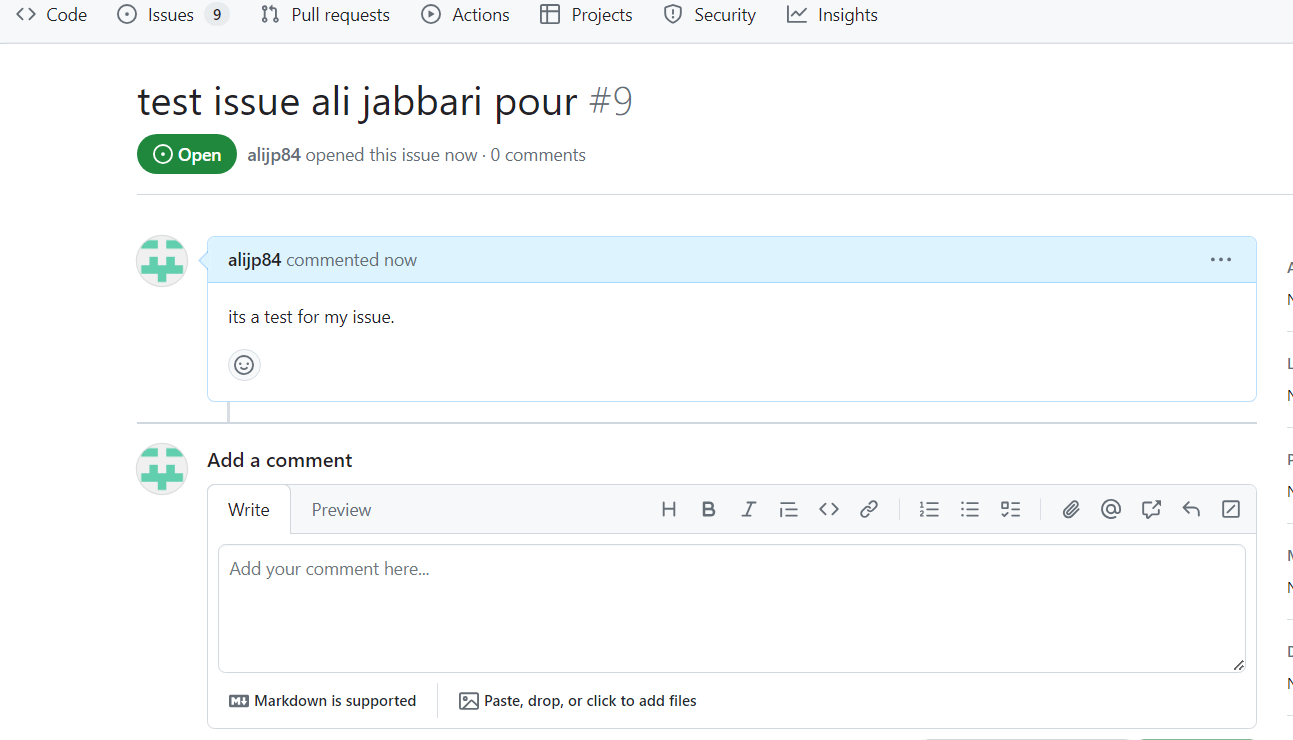
\includegraphics[width=1/textwidth]{screne issue.png}
\caption{issue ali jabbari pour}
\end{figure}
\end{document}

